
\documentclass[12pt, a4paper]{article}
\usepackage{amssymb}
\usepackage[authoryear, round]{natbib}
\usepackage{amsthm}
\usepackage{amsmath}
\usepackage{algorithm}
\usepackage{algpseudocode}
\usepackage{float}
\usepackage[titletoc,toc,title]{appendix}
\usepackage{fullpage} %can add [cm] to have more margin
\usepackage{graphicx}

\theoremstyle{definition}
\newtheorem{defn}{Definition}[section]

\begin{document}

\title{
	{
	Feature Generation by Recursive Induction%mby change to Induction-Based learning?
	}\\
	%Automated Feature Generation using Inductive Learning over Feature Values}\\
}
\author{
    {A M.S.c research proposal by Lior Friedman}\\
    {Under the supervision of Prof. Shaul Markovitch}
}

\maketitle

\section{Introduction}
\label{sec:Intro}
In recent decades, we have seen an increasing prevalence of machine learning techniques used in a wide variety of fields such as medical diagnosis, vision, and biology.
Most machine learning methods assume a given set of labeled examples represented by a set of
pre-defined features. These methods have proven to be successful when a collection of good,
distinguishing features is available.
In many real-world applications, however, the given set of features is not sufficient for inducing a high quality classifier.

One approach for overcoming the difficulty resulting from an insufficiently expressive set of features, is to generate new features.  Most feature generation algorithms produce new features by combining the original ones in various ways.  For example, the LFC algorithm \citep{ragavan1993complex} combines the original feature using logical operators.  The LDMT algorithm \citep{utgo1991linear} uses linear combinations of the original features to construct more informative ones.  The FICUS algorithm \citep{markovitch2002feature} presents a general framework for using any set of constructors to combine features.

Recently, there has been a strong trend of utilizing \emph{Deep Learning} \citep{lecun1998gradient, bengio2009learning} as a feature generation technique. These methods essentially form combinations and transformations on pre-defined features in a semi-supervised manner, thus yielding new, more predictive features.
There are many good examples of this, such as the ones presented in \citet{plotz2011feature}, as well as \citet{kim2013deep}.

While feature combination has proven to enhance the performance of induction algorithms, there are many cases where a mere combination of existing features is not enough.  To that extent, a different approach for generating features has been devised.  This approach aims to incorporate additional knowledge from external sources in order to construct new and informative features.
\citet{gabrilovich2007computing} for example, present a method for generating features that are based on Wikipedia concepts. \citet{jarmasz2012roget} presents a method for utilizing lexical links between words to generate features.

In the case where this external knowledge is organized as a set of relations between entities, several methods can be used. One such method is using \emph{Inductive Logic Programming} \citep{muggleton1991inductive} to generate features, in a process referred to as \emph{upgrading} \citep{van2001upgrade}. This process is demonstrated through the ICL algorithm (same paper), an algorithm that uses a refinement graph to search for logical formulae which serve as features. The SGLR algorithm \citep{popescul200716} extends this idea to numerical features, generated using aggregation-based techniques, and then utilizes regression for inference.

In this work, we present a new methodology for using relational knowledge for feature generation.  Our algorithm uses common induction algorithms over sets of feature values, resulting in classifiers which are then used as new features.
Such classifier-based features can effectively capture complex relationships that are difficult to discover using existing feature-generation methods.

As an example of the potential use of such an approach, consider the following:
Suppose we are given medical records of patients containing name, country of origin as well as medically relevant information.
Our task is to identify patients with high risk of developing a \emph{genetic} disease, which is more common in warm countries as well as countries with a lower GDP.
The original set of features is not sufficient for inducing the target concept.  Assume, however, that we have access to an external knowledge base, containing, among others, relations specifying information about countries and connecting last names with country of origin.
Our method would first formulate a new induction problem where the positive examples are last names of high-risk patients, and then, through a recursive process, formulate a new problem where the positive examples are countries of origin corresponding to last names of high risk patients. The resulting classifier could then be used as a regular binary feature when classifying patients, allowing us to capture the genetic component of the disease through the last name. While traditional feature generation methods could find some relation-based trends, they would struggle to find the above relationship, as it is too complex.


\begin{figure}[H]
    \centering
    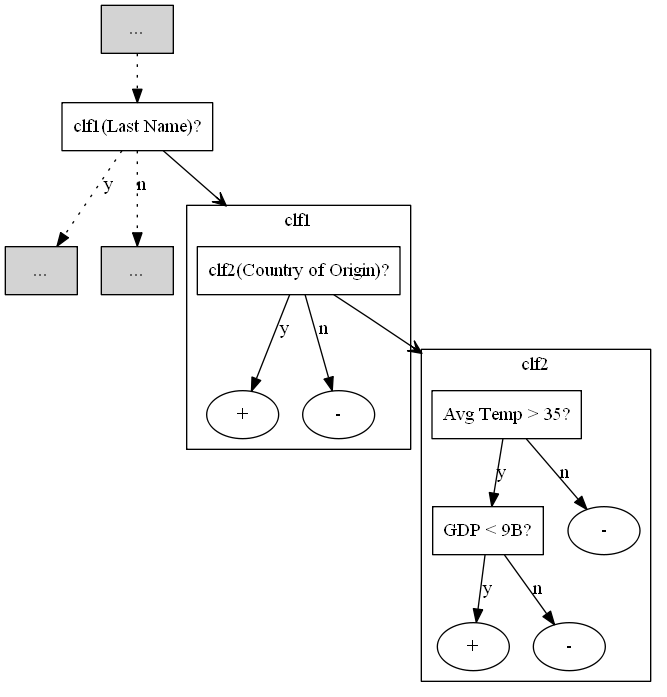
\includegraphics[scale=0.3, keepaspectratio=true]{output.png}
    \caption{An single node in the decision tree. Note that the split is made by calling an additional classifier (which is created using relational data) on the value of a feature.}
    \label{fig:example}
\end{figure}


%%%%%%%%%%%%%%%%%%%%%%%%%%%%%%%%%%%%%%%%%%%%%%%%%%%%%%%%%%
\section{Background} \label{background}
%%%%%%%%%%%%%%%%%%%%%%%%%%%%%%%%%%%%%%%%%%%%%%%%%%%%%%%%%%

One of the earliest methods of utilizing relational information, officially defined by \citet{muggleton1991inductive} and used even before then in the well-known FOIL algorithm \citep{quinlan1990learning}, is \emph{Inductive Logic Programming(ILP)}. This approach induces a set of first-order formulae
that define a good separation of the given training set. Originally, ILP methods searched the space of first-order formulae to find the appropriate classifier.
Over time, effort has been made to allow the usage of traditional propositional algorithms such as ID3 \citep{quinlan1986} over this domain.

One major attempt at adding relational knowledge to induction methods was \emph{propositionalization} \citep{kramer2000bottom}: Since we wish to allow the use of first-order predicates in propositional methods, we create possible (non recursive) first-order predicates in a process known as refinement search.
We define a graph of possible first-order formulae by selecting an initial relation and allowing one of two possible refinement operators: The first operator is binding a single variable in the formula by assigning a constant value to it, and the second is binding a single variable using another relation.

These operators define a search space. For each formula, we can ask whether a given object satisfies it, giving us a binary query for the data. We often prefer to only use formulae with one unbound variable, as it allows a simpler satisfaction check.
It is important to note that each application of refinement operators yields a formula that is subsumed by the parent, meaning that any object satisfying the child formula will also satisfy its parent.

A major setback of this process is that it generates an impractically large number of features, most of which irrelevant.  To this end, \emph{upgrade} methods such as ICL \citep{van2001upgrade} were suggested, where instead of creating predicates a-priori, we do so during the training phase, allowing us to avoid searching non-promising refinements.

As a continuation to this trend, \citet{popescul200716} suggest SGLR, an upgrade method which allows the generation of non-binary attributes by using aggregation operators. Essentially, instead of simply checking whether a first-order predicate is satisfied, we perform aggregation over all objects which satisfy it. In addition, SGRL offers an initial insight into the issue of improving the search process by using Akaike's information criteria (AIC, see \citet{burnham2002model}) to select features based on complexity as well as predictive power.

Newer advances in the relational approach can be seen in the field of \emph{Statistical Relational Learning} \citep{blockeel2013statistical, nath2014learning} as well as the task of \emph{Collective Classification} \citep{kajdanowicz2013collective, laorden2012collective}. The general field of Statistical Relational Learning (and reasoning) deals in tasks where there is a complex, relational structure within the domain. Common tasks in the field are: Collective classification, link prediction and entity resolution between datasets. Of these, the most relevant to our domain is the task of collective classification, where relational information is used to infer labels of objects based on related objects. However, this relational information is not used for feature generation, but as a way to link objects within the target domain.

In recent years, a new resource in the form of Semantic Linked Data has begun to take form, as part of the Semantic Web project (see survey, \citet{bizer2009linked}). This resource has led to the creation of several new approaches designed to utilize this new, ontology-based representation of knowledge \citep{losch2012graph,rios2014statistical}.

To this end, there have been several efforts in utilizing Linked Data for Feature Generation \citep{cheng2011automated, paulheim2012unsupervised}. While these techniques offer some insight towards applying the knowledge within such an extensive knowledge base as features, they add them in an unsupervised manner, leading to the creation of an impractically large number of features, most of which are irrelevant, as seen in propositionalization methods. Due to this, they have difficulties handling complex relationships.


An interesting domain can be found in a well-known and well-explored task within the field of Natural Language Processing(NLP): the task of text classification.
The task of text classification involves assigning categories or labels to documents, based on their content. The potential labels/categories are given in advance, and we have a collection of labeled documents to use as a training set. This task has many practical applications, such as spam filtering, sentiment analysis and topic identification.

Until recent years, text classification systems represented text almost exclusively as a \emph{Bag of Words}, thus creating a vector space representation \citep{salton1983introduction,Wu:1981:CST:1013228.511759}. While this method offered simplicity, it had inherent limitations in terms of representation power.

A major breakthrough came in the form of the \emph{explicit sematic analysis} \citep{gabrilovich2006overcoming} method, which used semantic concepts extracted from knowledge sources such as Wikipedia as features. This technique allowed for a richer representation of the text, and has shown improvement over the Bag-of-Words representation for the task of text classification, especially in shorter texts.

%Final paragraph here to finish.
The goal of our work is to utilize Linked Data as a knowledge source for automatically generating features based on meaningful semantic concepts, thus improving existing machine learning algorithms. We intend to do so in a supervised manner to allow a better guided search over candidate features, based on a combination of complexity and predictive power. We will place focus on the domain of text classification as a natural application of our approach.

%%%%%%%%%%%%%%%%%%%%%%%%%%%%%%%%%%%%%%%%%%%%%%%%%%%%%%%%%%
\section{Proposed Solution}
%%%%%%%%%%%%%%%%%%%%%%%%%%%%%%%%%%%%%%%%%%%%%%%%%%%%%%%%%%

Let $O$ be a set of objects. Let $Y=\{0,1\}$ be a set of labels (we assume binary labels for ease of discussion). Let $S=\{(o_{1},y_{1}),\ldots,(o_{m},y_{m})\}$ be a set of labeled examples such that $o_{i}\in O, y_{i}\in Y$. Let $F=\{f_{1},\ldots,f_{n}\}$ be a \emph{feature map}, a set of \emph{feature functions} $f_{i}:O\rightarrow Dom_{i}$.  This definition implies a training set represented by feature vectors: $\{ (\langle f_1(o_i),\ldots,f_n(o_i)\rangle, y_i) | (o_i,y_i) \in S\}$.

Given a set of relations $\bar{R}=\{R_{1},\ldots,R_{t}\}$ with arity of $n_{j}$ ($j=1\ldots k$), we can assume \text{w.l.o.g} that the first argument is a key. For each relation $R_{j}$ we define $n_{j}-1$ new binary relations where each of the first elements is the key and the second one is another column.
Let ${\cal R}=\{R_{1},\ldots,R_{k}\}$ be such set of binary relations, where $R_{i}$ is defined over $K_{i}\times D_{i}$. These relations can thus be seen as functions $R_{i}: K_{i}\rightarrow D_{i}$.

\begin{defn}
A \emph{supervised feature generation algorithm} $A$ using relations is an algorithm that given $\langle S,F,{\cal R} \rangle$, creates a new feature map $F_{\cal R}=\{f'_{1},\ldots,f'_{l}\}$.
\end{defn}

We would like the new hypothesis space, defined over $F_{\cal R}$, to be one that is both rich enough to provide hypotheses with a lower loss than those in the original space, as well as simple enough that the learning algorithm used will be able to find such good hypotheses given training data.
We would also like there to be connections between $F$ and ${\cal R}$, meaning some of the feature values of features in $F$ (when applied to objects in $S$) also exist within relations in $\cal R$.

We propose a general feature generation algorithm using additional knowledge on feature values.
Given an original feature $f_{i}$ with domain $Dom_i$, our algorithm will formulate a new learning task trying to separate values in $Dom_i$ appearing in positive examples of the original learning task from those appearing in negative ones.  The result of the new learning task will be a classifier
$h_{i}:Dom_{i}\rightarrow \{0,1\}$ that can label feature values of $f_{i}$. We can then define a new binary feature $f'_{i}(x)=h_{i}(f_{i}(x))$.
We name this algorithm \emph{Binary-RFG}, as it generates binary features (For pseudo-code, see appendix \ref{app:2}.

In order to explain how we create such $h_{i}$, let us consider a single step of the feature generation algorithm.
Given a feature $f_{i}$, we define the set of all its value in the training set $S$ as $v_i(S) = \{v | (o,y) \in S, f_{i}(o)=v\}$. In the intro example, for instance, $v_i(S)$ will be the set of all last names of patients.
We now formulate a new learning problem with the new training set
$\hat{S_i} = \{ (v, label(v)) | v \in v_i(S) \}$.
The labeling function can be, for example, defined as
the majority label: $label(v)=majority(\{y_k| \left(o_k,y_k \right) \in S, f_{i}(o_k)=v\})$.

To define a feature map over the new training set $\hat{S}$, we look for all relations in $\cal R$ where the domain of the key argument contains $v_i$:
${\cal G}(S,{\cal R}) = \left\{ r \in {\cal R} | v_i(S) \subseteq \{x_1 | (x_1,x_2) \in r\}\right\}$. In the intro example, one such $r$ can be a relation mapping last names to countries of origin. We then use ${\cal G}$ as a feature map for $\hat{S_i}$.
Solving this new learning problem on $\hat{S_i}, {\cal G}(S,{\cal R})$ yields our classifier $h_{i}$.
Note that during the process of learning $h_{i}$, we can once again call the feature generation procedure to generate useful features for \emph{that} task, hence the recursive aspect of the process.

Through the above process, we can define a tree of possible domains to search over as follows:
\begin{defn} Domain:\\%defined recursivly. add that we can do ANY transform G using S,R,F
$S$ is a domain.
If $\bar{S}$ is a domain, then for any function $G_{\bar{F},\bar{R}}: O\rightarrow Dom_i$, $\bar{S'}=\{(v_i,label(v_i)|(o,y)\in \bar{S}, v_i=G_{\bar{F},\bar{R}}(o)\}$ is also a domain.
\end{defn}
The result is a process that bears some similarity to that of search over a refinement graph \citep{dvzeroski2001introduction,van1998completeness}.
Given sufficient resources, we could potentially search this tree exhaustively during the learning process. In most practical cases, however, an exhaustive search proves intractable, and we must select a search strategy over this tree.

The unique contributions of this method are as follows:
\begin{itemize}
    \item By moving our domain space when constructing a new problem, we essentially look at the problem from another perspective, which allows for the discovery of complex relationships.
    \item The process of re-labeling allows noise reduction and emphasizes more general trends within the data that may be harder to otherwise notice.
    \item We can exploit the power of existing, well-developed learning algorithms when we create a classifier, and possibly use different ones as we take recursive steps.
\end{itemize}

We can also consider a \emph{local} variation of our algorithm, where instead of finding features that perform well on the entirety of the data, we find features which are good on specific subsets. To do so, we use the above method to find a single binary feature, and apply it to the objects. Then, we split the objects to those labeled positive and those labeled negative. This process can then be repeated on each subset to increase the granularity of the generated features at the cost of a smaller, potentially biased training set.

Finally, we note that the local variation yields an algorithm that can easily be made into an \emph{anytime algorithm}: an algorithm that given more allotted computation time to learn, will produce results of higher quality \citep{zilberstein1996using}. You may see the anytime version for the case of decision trees as the classifier in appendix \ref{app:3}

%\section{Practical Considerations}
%Note that in order to classify using traditional methods, we must transform feature values appropriately, for example, we can derive binary feature values by using $q_{g_{j},c}(x)=\{\begin{array}{l l}
%            1 & \quad c\in g_{j}(x)\\
%            0 & \quad \text{otherwise} \end{array}$
%If relation is not a function->can be made function by set

\section{Research Questions}
Listed below are several interesting and potentially challenging research questions we intend on exploring during our work:
\begin{itemize}
    \item \emph{Cutoff strategies and threshold criteria.} We must define good stopping criteria for determining whether a resulting classifier created by the algorithm is likely to yield a good feature. We intend to explore several criteria, including Information-Gain ratio\citep{quinlan1986} and Akaike's corrected information criterion(see \citet{burnham2002model}). We must also consider the case of limited resources as a consideration, evaluating the gain from an additional recursive step against the computational cost of doing so. %AIC estimates same thing as Cross-Val: out of sample deviation. BIC estimates Minimum description length(model complexity)
        %read more on claims of correlation between AIC with LOO crossval and BIC with K-Fold crossval. does this mean I CAN use BIC?
        %update: AIC assumes true model not an option, and picks best approx candidate. BIC assumes true model exists as candidate, tries to find it. both CAN be used.
        %Conclusion: try both...most of the time they agree anyway
    \item \emph{Expansions to non-binary features.} The algorithm as written generates binary features. While it is not hard to arrive at non-binary features by applying aggregation based methods as in SGLR \citep{popescul200716}, it may be wise to explore other options to do so.
    \item \emph{Expansion of considered feature values.} At its current form, the algorithm is not designed to make use of numeric features. Such feature values must be handled differently than the ones we currently consider. We intend to consider several approaches to this.
    \item \emph{Labeling recursive problems.} A prevalent and highly interesting question is that of labeling examples within the constructed problem. In other words, how do we define $label(v)$ for $v_i(S)$? We intend on comparing the following methods in an empirical manner:
        \begin{itemize}
            \item Use only elements $v\in Dom_i$ which are consistent, meaning $|\{y|R(o)=v \wedge (o,y)\in S\}|=1$. The resulting label is thus that label.
            \item Take the majority of labels for all objects in $o\in O$ where $R(o)=v$. Generally any weighted averaging over the labels works here, but majority is the most immediate.
            \item Choosing a middle ground: Take a weighted average of labels, but only if this average is significantly (in the statistical sense) different than the result of a random labeling. Intuitively, this means we intend on choosing elements where the majority leans significantly towards a specific label. This helps eliminate weak majority trends in the data by treating them as noise.
        \end{itemize}
        Another aspect to consider is that we may choose to change the set of labels itself when moving between domains.
    \item \emph{Anytime expansion for other settings.} In this work, we consider the anytime setting using decision trees as a classifier. This choice yields a conceptually simple algorithm and means our generated features are highly relevant. To the best of our knowledge, there are few works regarding usage of external knowledge for anytime learning, with the most recent work found being the one presented in \citet{lindgren2000anytime}. Therefore, there is a highly vested interest in applying this anytime approach to other cases in an effective, efficient manner.
\end{itemize}

\section{Evaluation}
In order to measure the performance and significance of this approach, we intend to empirically evaluate its performance for the domain of document classification. We intend to look at several datasets, ranging from classical, often used datasets such as 20 newsgroups \citep{Lang95} and OHSUMED \citep{hersh1994ohsumed} to more modern ones such as Reuters Corpus Volume I(RCV1) \citep{lewis2004rcv1} and TechTC \citep{davidov2004parameterized}. For Semantic linked data, we first intend to use YAGO2\citep{hoffart2013yago2}. We will consider the usage conceptNet5 \citep{speer2012representing} as well.\\

We intend to compare the accuracy of our approach against the achievable accuracy without the use of feature generation, as well as the accuracy achievable by other feature generation methods such as \emph{ESA} \citep{gabrilovich2006overcoming} and \emph{FeGeLOD} \citep{paulheim2012unsupervised}.

We will place focus on decision trees and the basic, local algorithm, an instance which allows easier adaptation as well as interpretability.
In addition, we intend on measuring the anytime performance of its anytime variation compared to traditional anytime algorithms that do not make use of additional feature generation.

\bibliographystyle{plainnat}
\bibliography{document}

%\appendix
\begin{appendices}
\pagebreak

%\section{Basic-RFG algorithm} \label{app:1}
%\begin{algorithm}[H]
%$S=\{(o_{i},y_{i})\}$- set of labeled objects. We will mark $Ob$ the objects and $y$ the appropriate labels.
%
%$F$- A set of feature-functions.
%
%$\cal R$- A set of relations.
%
%$G$- A transformation function.
%
%$n$- Number of features to generate.
%
%$cond$- Stopping criteria.
%
%classifiers- An array of the classifier to be used at every level of the recursive process.
%
%\caption{Global-RFG}
%\label{code1}
%\begin{algorithmic}
%\Function{RFG}{S, F, R, G, n, classifiers, cond}
%\If {cond(S,F) or n $< 1$}
%    \State
%    \Return \Call {classifiers[0]}{F(Ob),y}
%\EndIf
%\State featureChosen= \Call {pickFeature}{S,F, n}
%\State newObjects= featureChosen(Ob)
%\State newLabels= \Call {label}{S,newObjects}
%\State newF= \Call {G}{S,F,R}
%\State newClassifier= \Call {RFG}{(newObjects,newLabels), newF, R, G, 1, classifeirs[1:], cond}
%\State newFeature= function(x): return \Call {newClassifier}{featureChosen(x)}
%\State
%\Return newFeature$\cup$ \Call {RFG}{S, F, R, G, n-1, classifiers, cond}
%\EndFunction
%
%\end{algorithmic}
%\end{algorithm}

\section{Binary-RFG algorithm} \label{app:2}
\begin{algorithm}[H]
$S=\{(o_{i},y_{i})\}$- set of labeled objects. We will mark $Ob$ the objects and $y$ the appropriate labels.

$F$- A set of feature-functions.

$\cal R$- A set of relations.

$n$- Number of features to generate.

$cond$- Stopping criteria.

classifiers- An array of the classifier to be used at every level of the recursive process.

\caption{Binary-RFG}
\label{code2}
\begin{algorithmic}
\Function{B-RFG}{S, F, R, n, classifiers, cond}
\If {cond(S,F) or n $< 1$}
    \State
    \Return classifiers[0](S,F)
\EndIf
\State featureChosen= \Call {pickFeature}{S,F}
\State newObjects= featureChosen(Ob)
\State newLabels= \Call {label}{S,newObjects}
\State newF= $\{R_{i}(newObjects)|R_{i}\in R, newObjects\cap D_{i}\neq\emptyset\}$
\State newClassifier= \Call {B-RFG}{(newObjects,newLabels), newF, R, 1, classifiers[1:], cond}
\State newFeature= function(x): return newClassifier(featureChosen(x))
\State
\Return newFeature$\cup$ \Call {B-RFG}{S, F, R, n-1, classifiers, cond}
\EndFunction

\end{algorithmic}
\end{algorithm}

\section{Anytime Local-Hierarchy-Binary-RFG Algorithm} \label{app:3}
\begin{algorithm}[H]
\caption{Anytime Tree-RFG}
\label{code3}
\begin{algorithmic}
\Function{Anytime-Improved-Tree}{currentTree, S, F, R, cond}
\If {timeout}
    \State
    \Return currentTree
\EndIf
\State nodeToImprove= \Call {pickNode} {currentTree, S}
\State newClassifier= \Call {B-RFG} {nodeToImprove.S, F, R, 1, [decisionTree], cond}
\State newFeature= function(x): return newClassifier(featureChosen(x))
\State posSet= $\{(x,y)\in$ nodeToImprove.S$|$newFeature(x)==1$\}$
\State negSet= S-posSet
\State newNode= \Call {makeNode} {newFeature, nodeToImprove.S, posSet, negSet}
\State currentTree.replace(nodeToImprove, newNode)
\State
\Return \Call {Anytime-Improved-Tree} {currentTree, S, F, R, cond}
\EndFunction

\end{algorithmic}
\end{algorithm}
\end{appendices}

\end{document}
